\let\negmedspace\undefined
\let\negthickspace\undefined
\documentclass[journal]{IEEEtran}
\usepackage[a5paper, margin=10mm, onecolumn]{geometry}
\usepackage{tfrupee} 
\setlength{\headheight}{1cm} 
\setlength{\headsep}{0mm}     

\usepackage{gvv-book}
\usepackage{gvv}
\usepackage{cite}
\usepackage{amsmath,amssymb,amsfonts,amsthm}
\usepackage{algorithmic}
\usepackage{graphicx}
\usepackage{textcomp}
\usepackage{xcolor}
\usepackage{txfonts}
\usepackage{listings}
\usepackage{enumitem}
\usepackage{mathtools}
\usepackage{gensymb}
%\usepackage{wasysym}
\usepackage{comment}
\usepackage[breaklinks=true]{hyperref}
\usepackage{tkz-euclide} 
\usepackage{listings}
\def\inputGnumericTable{}                                 
\usepackage[latin1]{inputenc}                                
\usepackage{color}                                            
\usepackage{array}                                            
\usepackage{longtable}                                       
\usepackage{calc}                                             
\usepackage{multirow}                                         
\usepackage{hhline}                                           
\usepackage{ifthen}                                           
\usepackage{lscape}
\usepackage{circuitikz}
\tikzstyle{block} = [rectangle, draw, fill=blue!20, 
    text width=4em, text centered, rounded corners, minimum height=3em]
\tikzstyle{sum} = [draw, fill=blue!10, circle, minimum size=1cm, node distance=1.5cm]
\tikzstyle{input} = [coordinate]
\tikzstyle{output} = [coordinate]
\renewcommand{\thefigure}{\theenumi}
\renewcommand{\thetable}{\theenumi}
\setlength{\intextsep}{10pt} % Space between text and floats
\numberwithin{equation}{enumi}
\numberwithin{figure}{enumi}
\renewcommand{\thetable}{\theenumi}

\begin{document}

\bibliographystyle{IEEEtran}
\vspace{3cm}

\title{4.7.24}
\author{EE25BTECH11032 - Kartik Lahoti}
\maketitle

\subsection*{Question: } 
Find the equation of line passing through the point $\brak{5,2}$ and perpendicular to the line joining the points $\brak{2,3}$ and $\brak{3,-1}$

\solution 

Given : 
\begin{table}[H]
    \centering
    \begin{tabular}{|c|c|}
\hline
\textbf{Name} & \textbf{Value} \\ \hline
$\vec{A}$ & $\myvec{2 & 1 \\0 & 3}$ \\ \hline
\end{tabular}

    \caption*{}
    \label{tab:placeholder_1}
\end{table}

Let , $\vec{X}$ be a vector on the Required Line

Direction Vector for the Line $\vec{AB}$ , 
\begin{align}
    \vec{B} - \vec{A} = \myvec{3 \\ -1} - \myvec{2 \\ 3} = \myvec{1 \\ -4}
\end{align}

Direction Vector for the Required Line in terms of $\vec{X}$ , 

\begin{align}
    \vec{X} - \vec{P} = \brak{\vec{X} - \myvec{5 \\ 2}}
\end{align}
Direction Vector for the Line $\vec{AB}$ is perpendicular to the required line
\begin{align}
        \therefore \brak{\vec{B} - \vec{A}}^{\top}\brak{\vec{X} - \myvec{5 \\ 2}} &= 0
\end{align}
\begin{align}
    \myvec{1 & -4}\brak{\vec{X} - \myvec{5 \\ 2}} &= 0
\end{align}

Hence, the desired equation is 

\begin{align}
    \myvec{1 & -4}\vec{X} = -3
\end{align}


\begin{figure}[H]
    \centering
    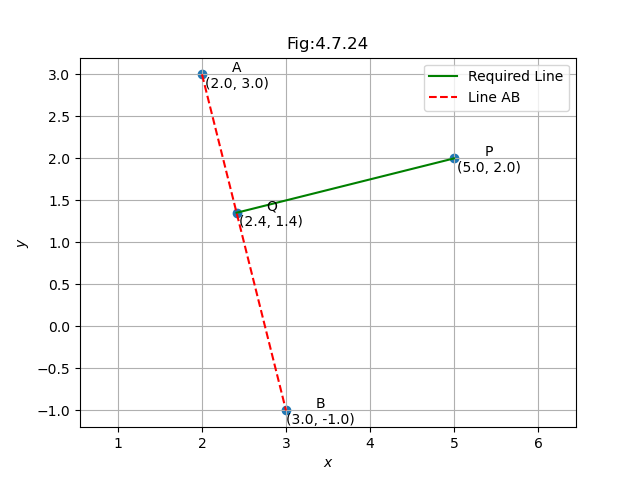
\includegraphics[width=1.0\columnwidth]{figs/perpendicular2.png}
    \caption*{}
    \label{fig:}
\end{figure}

\end{document}


